\documentclass[tikz,border=4pt]{standalone}
\usepackage{tikz}
\usetikzlibrary{positioning}
\definecolor{nebula}{HTML}{6366F1}
\definecolor{spark}{HTML}{14B8A6}
\begin{document}
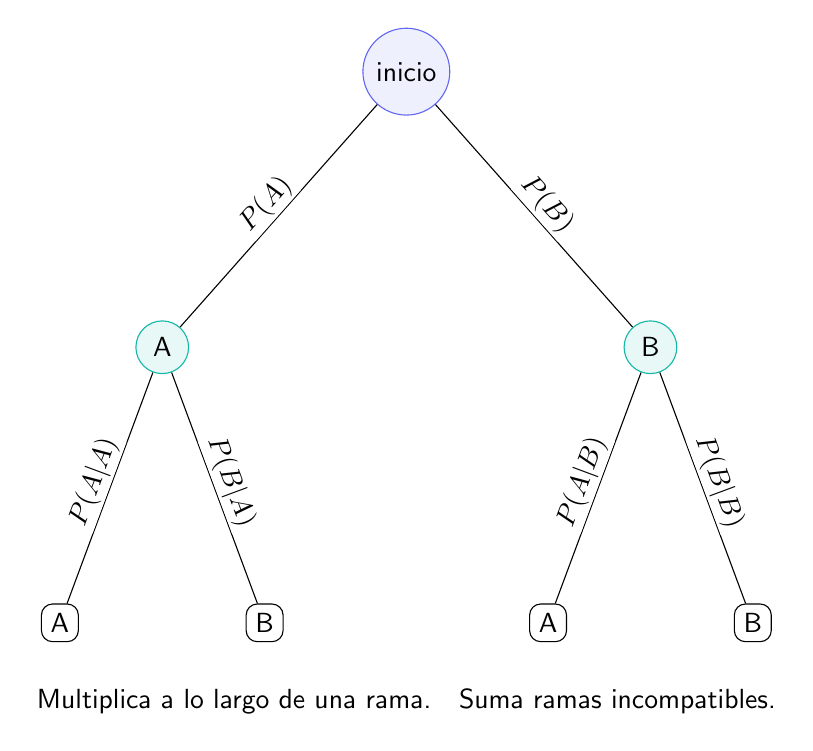
\begin{tikzpicture}[font=\sffamily,level distance=35mm,level 1/.style={sibling distance=62mm},level 2/.style={sibling distance=26mm}]
  \node[circle,draw=nebula,fill=nebula!10] {inicio}
    child {node[circle,draw=spark,fill=spark!10] {A}
      child {node[draw,rounded corners] {A} edge from parent node[midway,sloped,above,fill=white,inner sep=1pt] {$P(A|A)$}}
      child {node[draw,rounded corners] {B} edge from parent node[midway,sloped,above,fill=white,inner sep=1pt] {$P(B|A)$}}
      edge from parent node[midway,sloped,above,fill=white,inner sep=1pt] {$P(A)$}}
    child {node[circle,draw=spark,fill=spark!10] {B}
      child {node[draw,rounded corners] {A} edge from parent node[midway,sloped,above,fill=white,inner sep=1pt] {$P(A|B)$}}
      child {node[draw,rounded corners] {B} edge from parent node[midway,sloped,above,fill=white,inner sep=1pt] {$P(B|B)$}}
      edge from parent node[midway,sloped,above,fill=white,inner sep=1pt] {$P(B)$}};
  \node[align=center] at (0,-8.0) {Multiplica a lo largo de una rama.\quad Suma ramas incompatibles.};
\end{tikzpicture}
\end{document}
